\documentclass[conference,10pt]{IEEEtran}

\usepackage[T1]{fontenc}
\usepackage[utf8]{inputenc}
\usepackage[spanish,es-nodecimaldot]{babel}
\spanishplainpercent
\usepackage{amsmath,amssymb}
\usepackage{booktabs}
\usepackage{xcolor}
\usepackage{float}
\usepackage{graphicx}
\usepackage[american]{circuitikz}
\usetikzlibrary{babel}

\graphicspath{{img/}}

\definecolor{placeholder}{RGB}{110,110,110}
\newcommand{\completar}[1]{%
  \ifmmode\text{\color{placeholder}\itshape[Completar: #1]}%
  \else\textcolor{placeholder}{\textit{[Completar: #1]}}\fi}

\title{Informe: Circuitos Resistivos y Ley de Ohm\\
Práctica de Laboratorio No. 2}

\author{
  \IEEEauthorblockN{Maria Paula Mejía Vásquez, Cristian Alejandro Guarin Marin}
  \IEEEauthorblockA{
    Ingeniería Electrónica y de Telecomunicaciones\\
    Circuitos Eléctricos I -- Universidad de Antioquia\\
    Periodo 2026-2\\
    paula.mejia3@udea.edu.co, cristian.guarinm@udea.edu.co
  }
}

\begin{document}
\maketitle

\begin{abstract}
Este informe presenta el desarrollo de la Práctica de Laboratorio No. 2, en la que se verifican de manera experimental la ley de Ohm y las técnicas de simplificación de circuitos resistivos (serie, paralelo y transformación delta--estrella). Se comparan los resultados obtenidos en el preinforme, en la simulación con LTspice y en el montaje físico en protoboard para tres circuitos: una conexión puramente paralela, una puramente serie y una red mixta que requiere una transformación delta--estrella. Los tres conjuntos de resultados presentan una concordancia adecuada, con diferencias atribuibles principalmente a la tolerancia de los resistores comerciales y a la resistencia de contacto introducida por el montaje.
\end{abstract}

\begin{IEEEkeywords}
Ley de Ohm, circuitos resistivos, resistencia equivalente, conexiones serie-paralelo, transformación delta--estrella, LTspice.
\end{IEEEkeywords}

\section{Introducción}
La ley de Ohm y las reglas de asociación de resistores en serie y en paralelo permiten predecir el comportamiento de una red resistiva a partir de los valores nominales de sus componentes. Sin embargo, los valores reales de los resistores comerciales, las condiciones de la fuente de alimentación y la calidad de las conexiones en el montaje físico introducen diferencias respecto a los valores calculados teóricamente. En esta práctica dichas diferencias se cuantifican comparando tres etapas de un mismo análisis: el cálculo previo (preinforme), la simulación en LTspice y la medición directa sobre el montaje en protoboard, para tres circuitos de complejidad creciente.

\section{Objetivos}
\subsection{Objetivo general}
Verificar experimentalmente la ley de Ohm y la simplificación de circuitos resistivos en configuraciones serie, paralelo y mixta, contrastando los valores calculados, simulados y medidos.

\subsection{Objetivos específicos}
\begin{itemize}
  \item Medir con el multímetro los valores reales de los resistores empleados y compararlos con sus valores nominales.
  \item Simular en LTspice los tres circuitos propuestos y obtener la corriente y el voltaje suministrados por la fuente mediante un análisis de punto de operación (.op).
  \item Realizar el montaje físico de los tres circuitos en protoboard y medir la resistencia equivalente, el voltaje y la corriente de cada uno.
  \item Comparar los resultados de preinforme, simulación y montaje, e identificar las causas de las diferencias encontradas.
\end{itemize}

\section{Materiales y componentes utilizados}
Para el desarrollo de la práctica se emplearon los siguientes materiales: protoboard, multímetro, fuente de voltaje ajustada a $v_s=5~\mathrm{V}$, cables de conexión y cinco resistores de valores comerciales distintos, seleccionados dentro del rango de $330~\Omega$ a $4.7~\mathrm{k}\Omega$ con potencia de $1/4~\mathrm{W}$.

\begin{figure}[H]
  \centering
  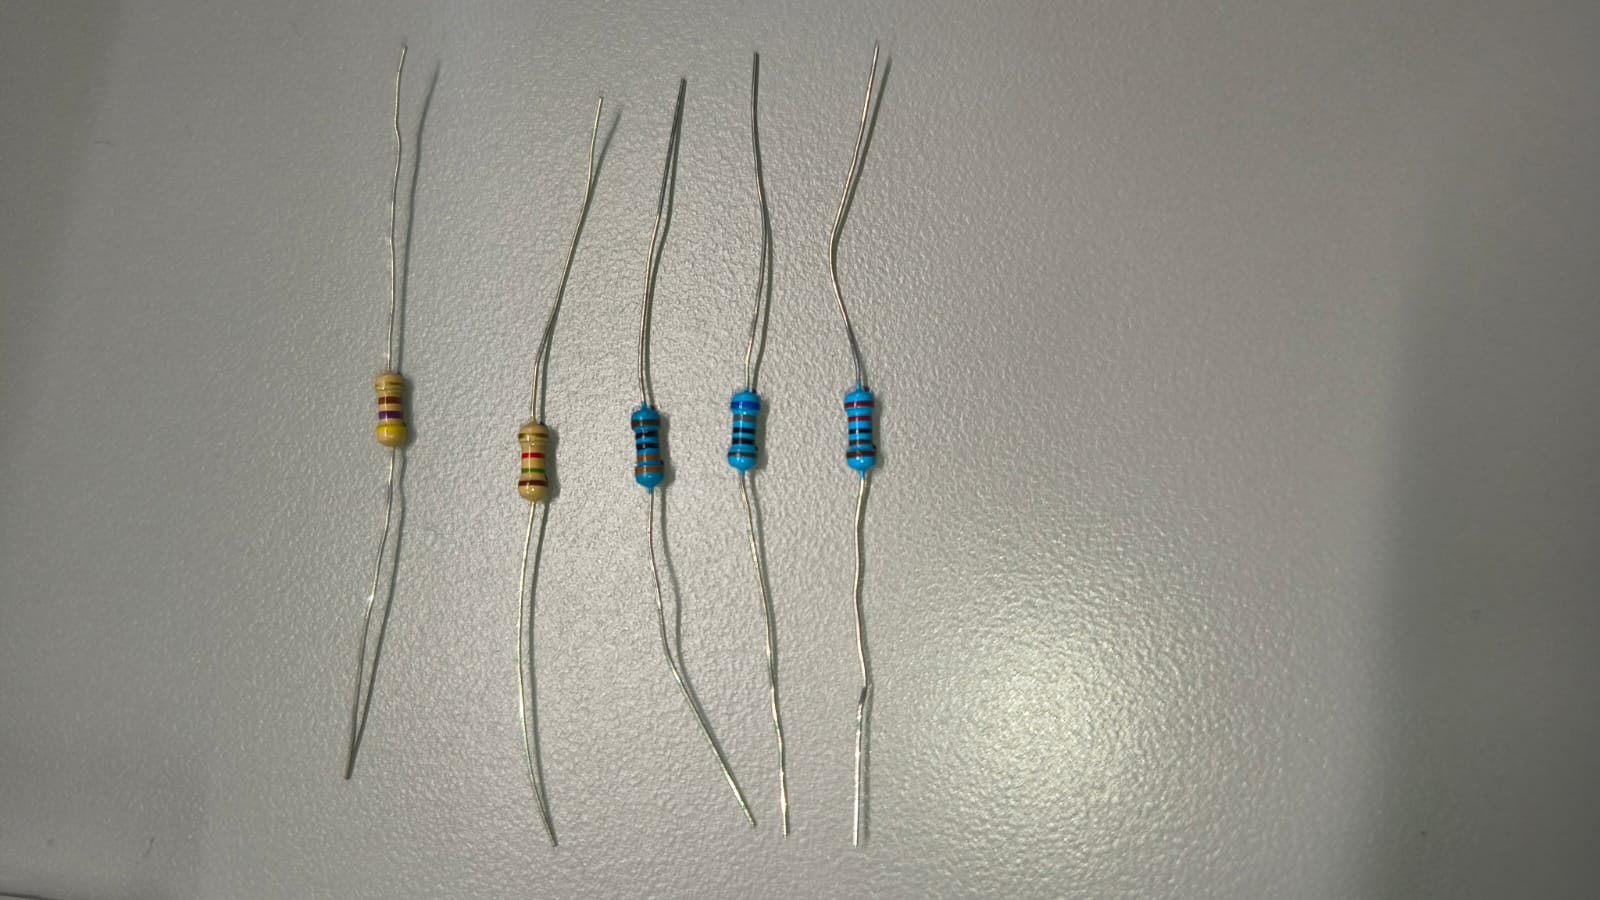
\includegraphics[width=0.85\linewidth]{resistores.png}
  \caption{Resistores $R_a$ a $R_e$ empleados en la práctica, donde se aprecia el código de colores de cada uno.}
  \label{fig:resistores}
\end{figure}

La Tabla~\ref{tab:medidas-resistencia} presenta el valor nominal de cada resistor, el valor medido con el multímetro antes del montaje de los circuitos, y el rango de valores esperado según su código de colores.

\begin{table}[H]
  \caption{Tabla Valores Medidos de Resistencia}
  \label{tab:medidas-resistencia}
  \centering
  \resizebox{\linewidth}{!}{%
  \begin{tabular}{cccccc}
    \toprule
    Resistor & Nominal ($\Omega$) & Medido ($\Omega$) & Tolerancia & Rango esperado ($\Omega$) & Dentro de rango \\
    \midrule
    $R_a$ & $680$  & $666$  & $1\,\%$ & $[673.2,\ 686.8]$   & No (\,$-1.06\,\%$\,) \\
    $R_b$ & $2200$ & $2137$ & $1\,\%$ & $[2178,\ 2222]$      & No (\,$-2.86\,\%$\,) \\
    $R_c$ & $470$  & $462$  & $5\,\%$ & $[446.5,\ 493.5]$    & Sí \\
    $R_d$ & $1500$ & $1500$ & $5\,\%$ & $[1425,\ 1575]$      & Sí \\
    $R_e$ & $330$  & $330$  & $1\,\%$ & $[326.7,\ 333.3]$    & Sí \\
    \bottomrule
  \end{tabular}}
\end{table}

\noindent Las tolerancias de la tabla corresponden a las anotadas en las mediciones de laboratorio (banda de tolerancia leída sobre cada resistor). Los resistores $R_c$, $R_d$ y $R_e$ midieron dentro de su rango nominal $\pm$ tolerancia. Los resistores $R_a$ y $R_b$, en cambio, midieron por debajo del límite inferior de su banda de $1\,\%$ (por $7.6~\Omega$ y $41~\Omega$, respectivamente); dado que ambos son resistores de precisión ($1\,\%$), esta pequeña desviación sugiere un error de calibración del multímetro empleado o una ligera deriva del valor del resistor, más que un defecto de fabricación, y no compromete el resto del análisis.

\section{Transformación delta--estrella y estrella--delta}
Una red de tres resistencias conectada en delta puede reemplazarse por una red equivalente en estrella entre los mismos tres terminales, y viceversa, conservando las corrientes y tensiones observables desde los terminales externos. Esta transformación se empleó para simplificar el circuito mixto de la Figura~\ref{fig:circuito-puente} (Sección~\ref{sec:figura4}), transformando la delta formada por $R_a$, $R_b$ y $R_c$ en su estrella equivalente.

Definiendo $S=R_a+R_b+R_c$, con $R_1$, $R_2$ y $R_3$ los brazos de la estrella hacia los nodos superior, izquierdo y derecho, respectivamente,
\begin{align}
  R_1 &= \frac{R_aR_b}{S}, &
  R_2 &= \frac{R_aR_c}{S}, &
  R_3 &= \frac{R_bR_c}{S}.
\end{align}

De forma análoga, definiendo $P=R_1R_2+R_2R_3+R_3R_1$, la transformación estrella--delta está dada por
\begin{align}
  R_a &= \frac{P}{R_3}, &
  R_b &= \frac{P}{R_2}, &
  R_c &= \frac{P}{R_1}.
\end{align}

El desarrollo completo de esta consulta, junto con los cálculos previos de los tres circuitos, se presentó en el preinforme de esta práctica.

\section{Circuito de la Figura 2: conexión en paralelo}
\setcounter{figure}{1}
\begin{figure}[H]
  \centering
  \begin{circuitikz}[scale=0.72, transform shape]
    \draw
      (0,0) to[battery1,l_=$v_s$] (0,3)
      -- (5.4,3)
      (0,0) -- (5.4,0)
      (1.8,3) to[R,l=$R_a$] (1.8,0)
      (3.2,3) to[R,l=$R_b$] (3.2,0)
      (4.6,3) to[R,l=$R_c$] (4.6,0);
    \draw[->] (0.45,3.35) -- node[above] {$i$} (1.35,3.35);
  \end{circuitikz}
  \caption{Elementos circuitales en paralelo.}
  \label{fig:circuito-paralelo}
\end{figure}

Los tres resistores empleados fueron $R_a=680~\Omega$, $R_b=2200~\Omega$ y $R_c=470~\Omega$, con una fuente $v_s=5~\mathrm{V}$. En el preinforme se calculó $R_{\mathrm{eq}1}=246.74~\Omega$ y $i_1=20.26~\mathrm{mA}$.

\begin{figure}[H]
  \centering
  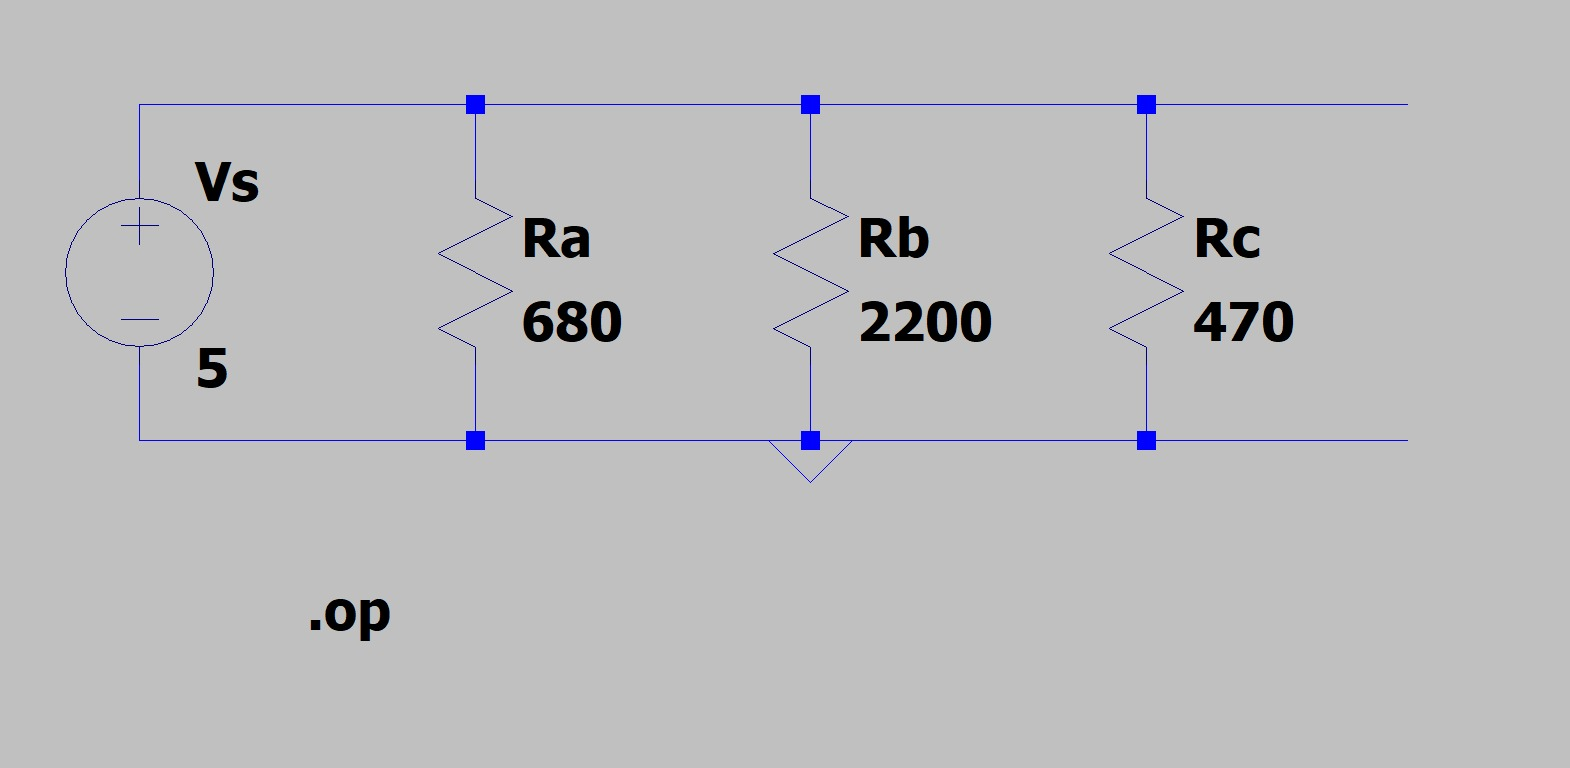
\includegraphics[width=\linewidth]{esquematico_fig2.jpeg}
  \caption{Esquemático simulado en LTspice del circuito de la Figura~\ref{fig:circuito-paralelo}: se identifica porque muestra $R_a=680~\Omega$, $R_b=2200~\Omega$ y $R_c=470~\Omega$ conectados en paralelo entre los mismos dos nodos.}
  \label{fig:esquematico-fig2}
\end{figure}

\begin{figure}[H]
  \centering
  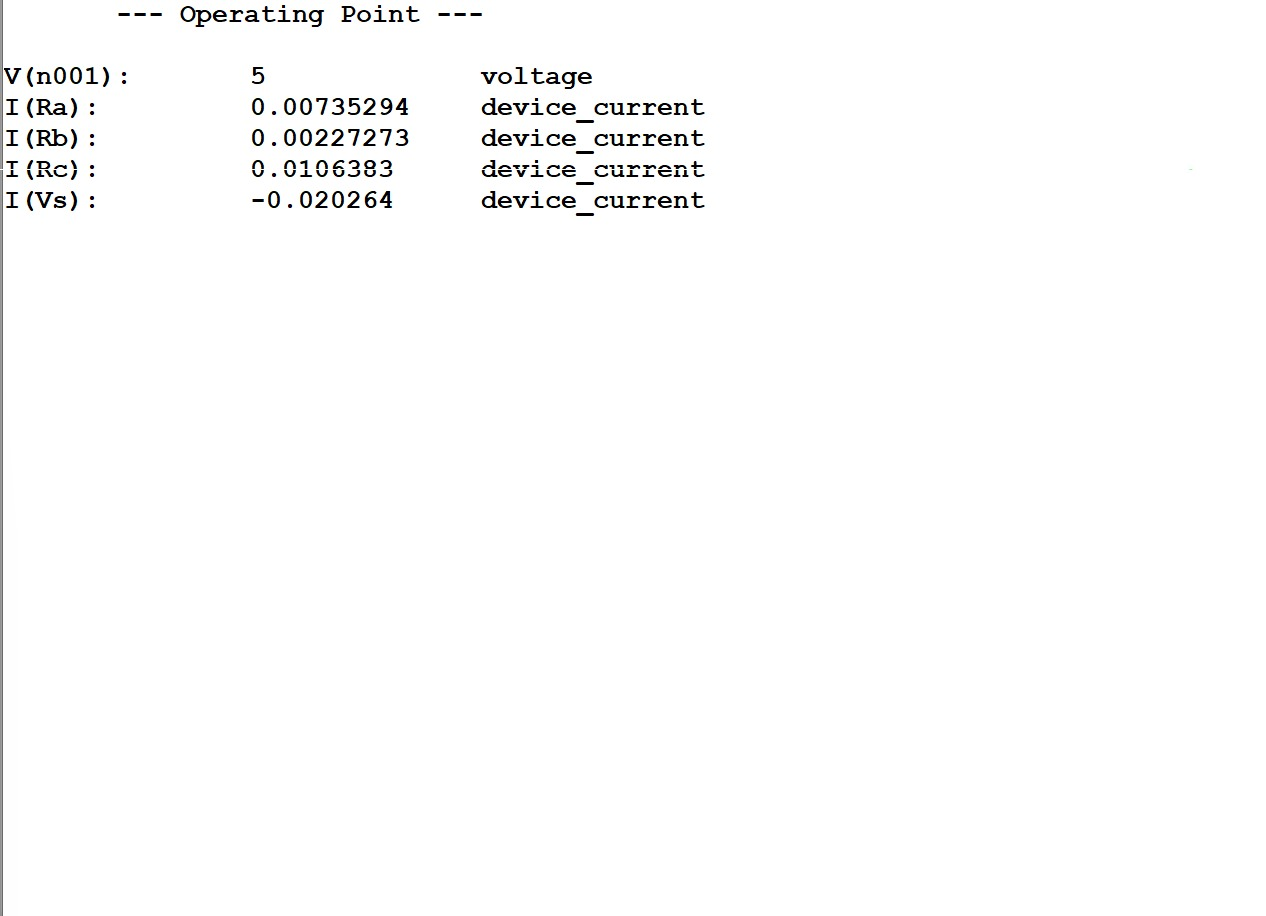
\includegraphics[width=0.85\linewidth]{resultados_fig2.jpeg}
  \caption{Resultados del análisis de punto de operación (.op) para el circuito de la Figura~\ref{fig:circuito-paralelo}: la suma de las tres corrientes de rama ($7.35+2.27+10.64~\mathrm{mA}$) reproduce la corriente total $i=20.26~\mathrm{mA}$ de la fuente, confirmando que corresponde a este circuito.}
  \label{fig:resultados-fig2}
\end{figure}

\begin{figure}[H]
  \centering
  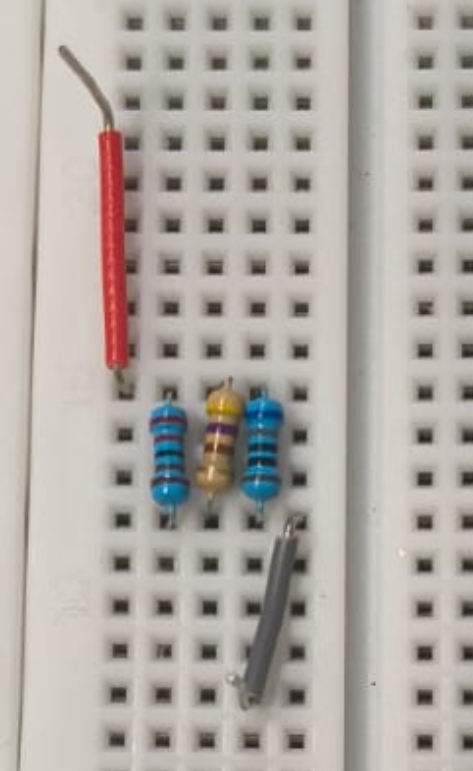
\includegraphics[width=0.85\linewidth]{montaje_fig2.png}
  \caption{Montaje físico del circuito de la Figura~\ref{fig:circuito-paralelo} en protoboard: los tres resistores quedan uno junto al otro compartiendo el mismo par de rieles, característico de una conexión en paralelo.}
  \label{fig:montaje-fig2}
\end{figure}

\begin{table}[H]
  \caption{Tabla Valores Circuito Figura 2}
  \label{tab:valores-fig2}
  \centering
  \resizebox{\linewidth}{!}{%
  \begin{tabular}{ccc|cc|ccc}
    \toprule
    \multicolumn{3}{c|}{Preinforme} & \multicolumn{2}{c|}{Simulación} & \multicolumn{3}{c}{Montaje} \\
    $R_{\mathrm{eq}1}$ ($\Omega$) & $v_s$ (V) & $i$ (mA) & $v_s$ (V) & $i$ (mA) & $R_{\mathrm{eq}1}$ ($\Omega$) & $v_s$ (V) & $i$ (mA) \\
    \midrule
    246.74 & 5.00 & 20.26 & 5.00 & 20.264 & 242.60 & 4.70 & 19.10 \\
    \bottomrule
  \end{tabular}}
\end{table}

\subsection*{Conclusiones}
Los resultados del preinforme y de la simulación coinciden prácticamente de forma exacta ($20.26~\mathrm{mA}$ frente a $20.264~\mathrm{mA}$), ya que la simulación emplea los mismos valores nominales de resistencia usados en el cálculo teórico. El valor medido en el montaje ($R_{\mathrm{eq}1}=242.6~\Omega$) es ligeramente menor que el calculado, lo cual es consistente con que los valores reales medidos de $R_a$, $R_b$ y $R_c$ (Tabla~\ref{tab:medidas-resistencia}) son levemente menores que los nominales. Adicionalmente, el voltaje medido en la fuente durante el montaje ($4.70~\mathrm{V}$) fue inferior al valor nominal de $5~\mathrm{V}$, lo que explica que la corriente medida ($19.1~\mathrm{mA}$) sea menor que la esperada a pesar de la menor resistencia equivalente. En conjunto, los tres resultados concuerdan dentro de un margen razonable, y las diferencias observadas se deben a la tolerancia de los resistores comerciales y a que la fuente no entregó exactamente $5~\mathrm{V}$ durante la medición.

\section{Circuito de la Figura 3: conexión en serie}
\begin{figure}[H]
  \centering
  \begin{circuitikz}[scale=0.72, transform shape]
    \draw
      (0,0) to[battery1,l_=$v_s$] (0,3)
      to[R,l=$R_a$] (2.2,3)
      to[R,l=$R_b$] (4.4,3)
      -- (4.4,0)
      to[R,l_=$R_c$] (2.2,0)
      -- (0,0);
    \draw[->] (1.15,3.45) -- node[above] {$i$} (2.05,3.45);
  \end{circuitikz}
  \caption{Elementos circuitales en serie.}
  \label{fig:circuito-serie}
\end{figure}

Empleando los mismos resistores $R_a=680~\Omega$, $R_b=2200~\Omega$ y $R_c=470~\Omega$ conectados ahora en serie, con $v_s=5~\mathrm{V}$, el preinforme arrojó $R_{\mathrm{eq}2}=3350~\Omega$ e $i_2=1.49~\mathrm{mA}$.

\begin{figure}[H]
  \centering
  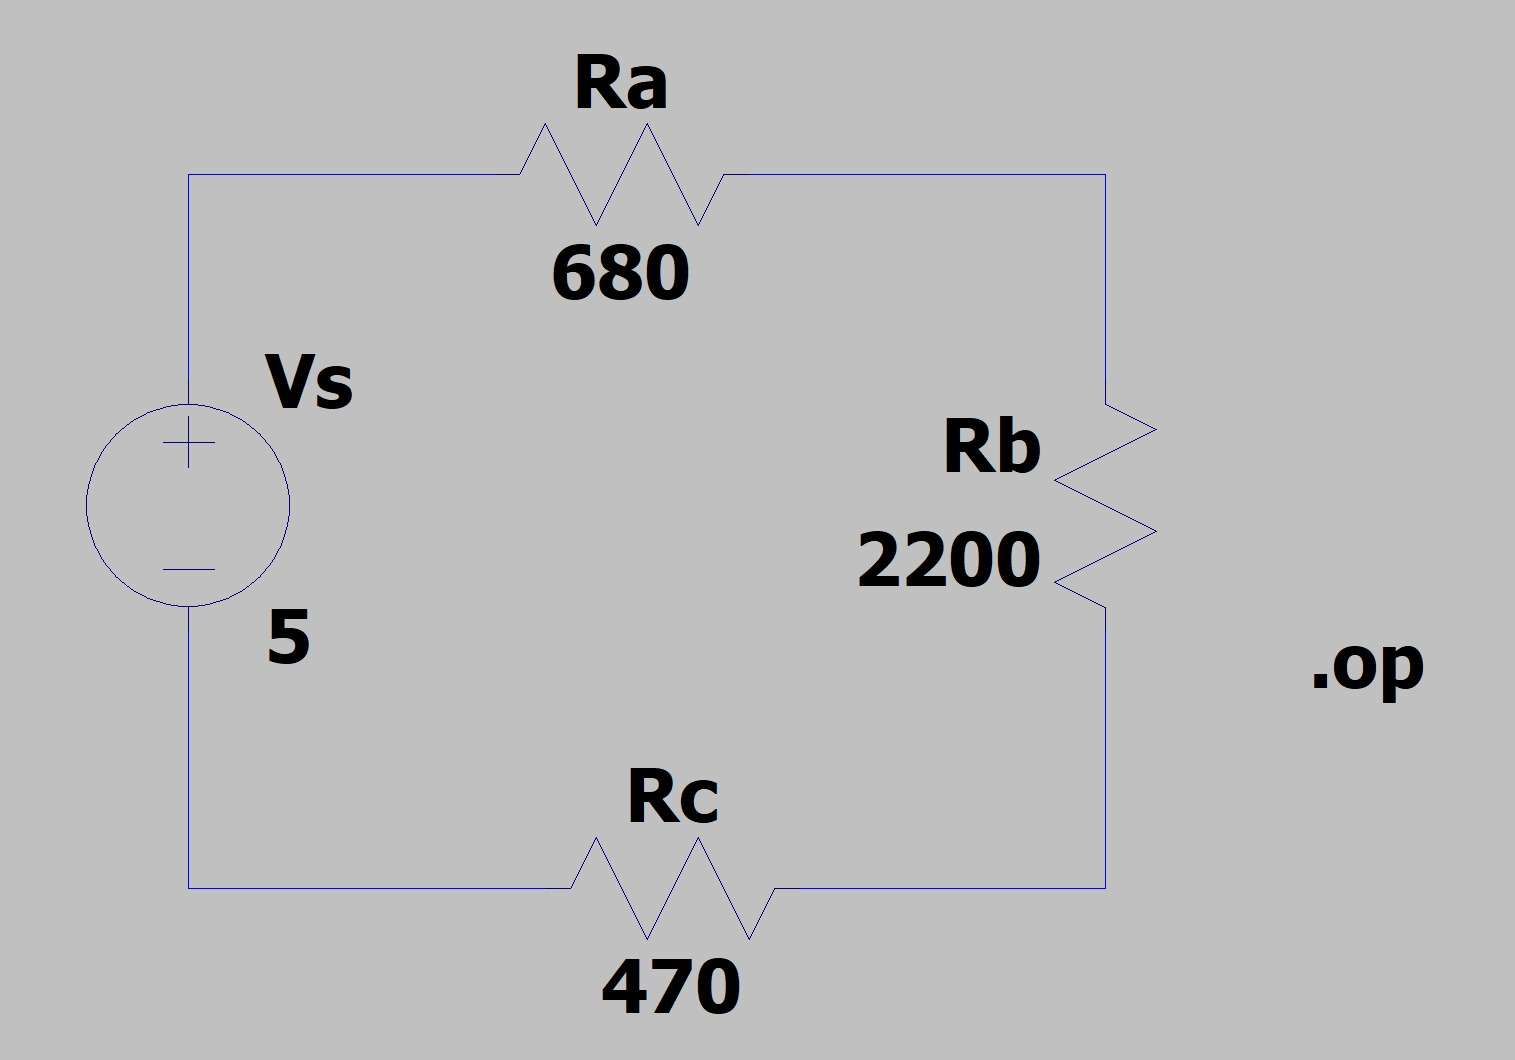
\includegraphics[width=\linewidth]{esquematico_fig3.jpeg}
  \caption{Esquemático simulado en LTspice del circuito de la Figura~\ref{fig:circuito-serie}: se identifica porque muestra $R_a$, $R_b$ y $R_c$ encadenados en un único lazo con la fuente, sin nodos compartidos entre ellos.}
  \label{fig:esquematico-fig3}
\end{figure}

\begin{figure}[H]
  \centering
  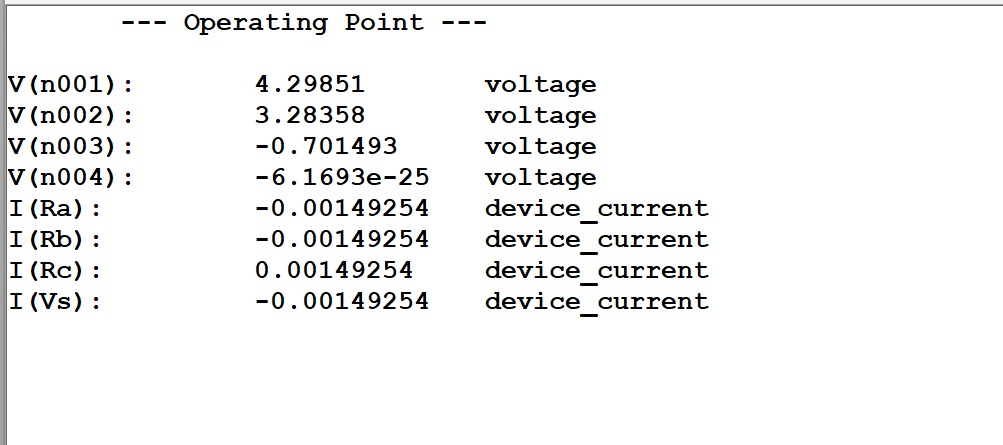
\includegraphics[width=0.85\linewidth]{resultados_fig3.jpeg}
  \caption{Resultados del análisis de punto de operación (.op) para el circuito de la Figura~\ref{fig:circuito-serie}: las cuatro corrientes reportadas ($R_a$, $R_b$, $R_c$ y $v_s$) son iguales entre sí ($1.49254~\mathrm{mA}$), como corresponde a una malla en serie.}
  \label{fig:resultados-fig3}
\end{figure}

\begin{figure}[H]
  \centering
  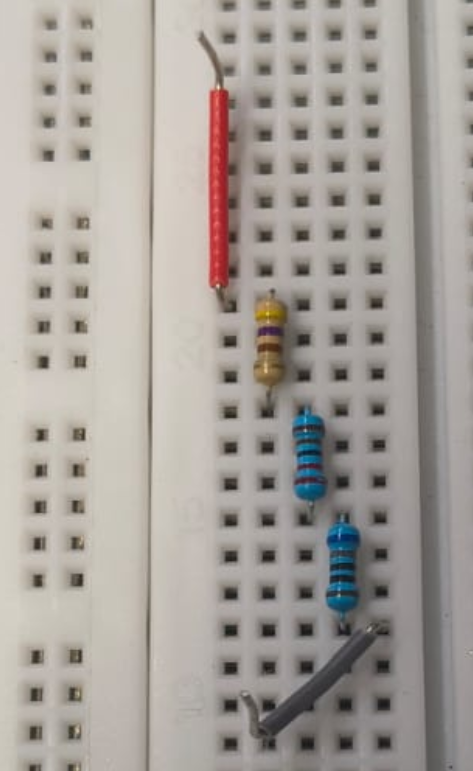
\includegraphics[width=0.85\linewidth]{montaje_fig3.png}
  \caption{Montaje físico del circuito de la Figura~\ref{fig:circuito-serie} en protoboard: los tres resistores quedan encadenados uno a continuación del otro en una misma columna, característico de una conexión en serie.}
  \label{fig:montaje-fig3}
\end{figure}

\begin{table}[H]
  \caption{Tabla Valores Circuito Figura 3}
  \label{tab:valores-fig3}
  \centering
  \resizebox{\linewidth}{!}{%
  \begin{tabular}{ccc|cc|ccc}
    \toprule
    \multicolumn{3}{c|}{Preinforme} & \multicolumn{2}{c|}{Simulación} & \multicolumn{3}{c}{Montaje} \\
    $R_{\mathrm{eq}2}$ ($\Omega$) & $v_s$ (V) & $i$ (mA) & $v_s$ (V) & $i$ (mA) & $R_{\mathrm{eq}2}$ ($\Omega$) & $v_s$ (V) & $i$ (mA) \\
    \midrule
    3350.00 & 5.00 & 1.49 & 5.00 & 1.493 & 3270.00 & 4.97 & 1.49 \\
    \bottomrule
  \end{tabular}}
\end{table}

\subsection*{Conclusiones}
Al igual que en el circuito paralelo, el preinforme y la simulación prácticamente coinciden ($1.49~\mathrm{mA}$ frente a $1.493~\mathrm{mA}$). En el montaje, la resistencia equivalente medida ($3270~\Omega$) resultó levemente menor que la nominal ($3350~\Omega$), y el voltaje de la fuente ($4.97~\mathrm{V}$) también estuvo por debajo del valor ideal. Sin embargo, ambos efectos se compensan parcialmente: al ser una configuración en serie, la corriente medida ($1.49~\mathrm{mA}$) resultó prácticamente idéntica a la calculada y simulada. Esto confirma que, para esta configuración, la ley de Ohm predice adecuadamente el comportamiento del circuito y que las pequeñas variaciones en los valores reales de los resistores y en el voltaje de la fuente no afectan significativamente el resultado final.

\section{Circuito de la Figura 4: red resistiva mixta}
\label{sec:figura4}
\begin{figure}[H]
  \centering
  \begin{circuitikz}[scale=0.72, transform shape]
    \draw
      (0,0) to[battery1,l_=$v_s$] (0,4)
      -- (1.7,4)
      (1.7,4) -- (4.6,4)
      (1.7,4) to[R,l=$R_a$] (1.7,2)
      to[R,l=$R_d$] (1.7,0)
      (4.6,4) to[R,l_=$R_b$] (4.6,2)
      to[R,l_=$R_e$] (4.6,0)
      (1.7,2) to[R,l=$R_c$] (4.6,2)
      (4.6,0) -- (0,0);
    \draw[->] (0.45,4.35) -- node[above] {$i$} (1.35,4.35);
  \end{circuitikz}
  \caption{Circuito que requiere una transformación delta--estrella o viceversa.}
  \label{fig:circuito-puente}
\end{figure}

Para este circuito se emplearon los cinco resistores disponibles: $R_a=680~\Omega$, $R_b=2200~\Omega$, $R_c=470~\Omega$, $R_d=1500~\Omega$ y $R_e=330~\Omega$, con $v_s=5~\mathrm{V}$. Transformando la delta formada por $R_a$, $R_b$ y $R_c$ en su estrella equivalente ($R_1=446.567~\Omega$, $R_2=95.403~\Omega$, $R_3=308.657~\Omega$), el preinforme obtuvo $R_{\mathrm{eq}3}=902.649~\Omega$ e $i_3=5.539~\mathrm{mA}$.

\begin{figure}[H]
  \centering
  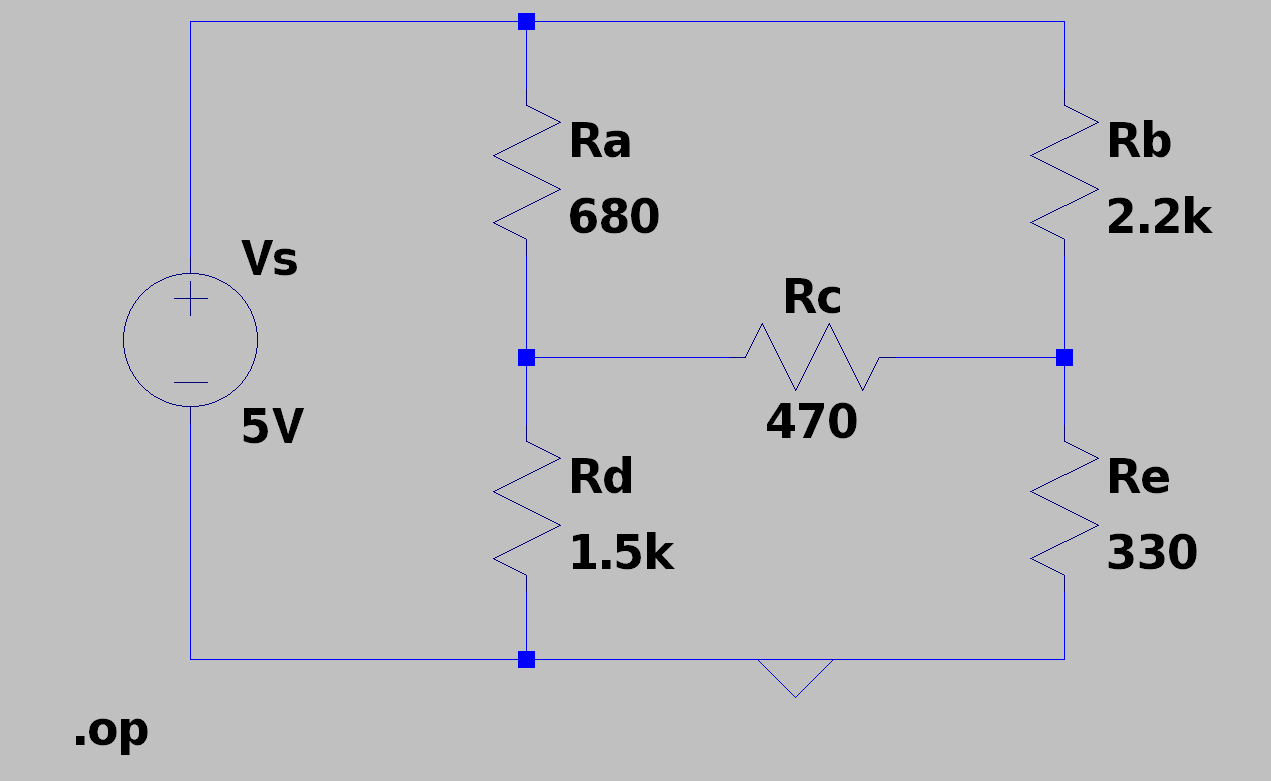
\includegraphics[width=\linewidth]{esquematico_fig4.png}
  \caption{Esquemático simulado en LTspice del circuito de la Figura~\ref{fig:circuito-puente}: se identifica por ser el único de los tres que emplea los cinco resistores ($R_a$ a $R_e$) en la topología de puente.}
  \label{fig:esquematico-fig4}
\end{figure}

\begin{figure}[H]
  \centering
  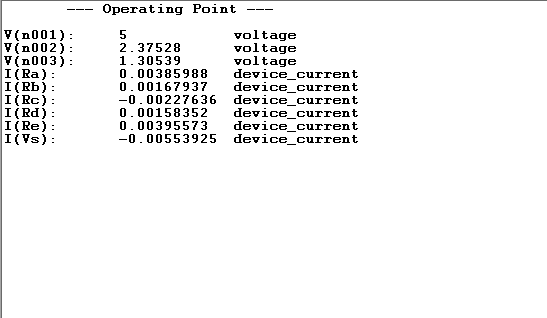
\includegraphics[width=0.85\linewidth]{resultados_fig4.png}
  \caption{Resultados del análisis de punto de operación (.op) para el circuito de la Figura~\ref{fig:circuito-puente}: reporta las cinco corrientes de rama ($R_a$ a $R_e$) y tres tensiones de nodo, y $|I(v_s)|=5.539~\mathrm{mA}$ coincide con el $i_3$ calculado en el preinforme, confirmando la correspondencia con este circuito.}
  \label{fig:resultados-fig4}
\end{figure}

\begin{figure}[H]
  \centering
  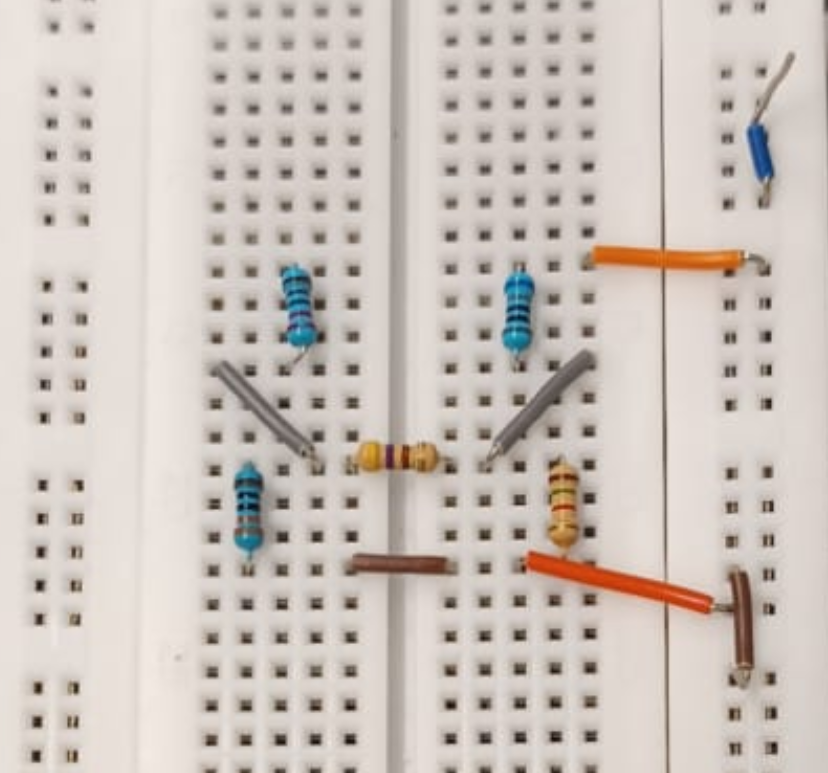
\includegraphics[width=0.85\linewidth]{montaje_fig4.png}
  \caption{Montaje físico del circuito de la Figura~\ref{fig:circuito-puente} en protoboard: es el único montaje con los cinco resistores y varios cables adicionales formando la topología de puente.}
  \label{fig:montaje-fig4}
\end{figure}

\begin{table}[H]
  \caption{Tabla Valores Circuito Figura 4}
  \label{tab:valores-fig4}
  \centering
  \resizebox{\linewidth}{!}{%
  \begin{tabular}{ccc|cc|ccc}
    \toprule
    \multicolumn{3}{c|}{Preinforme} & \multicolumn{2}{c|}{Simulación} & \multicolumn{3}{c}{Montaje} \\
    $R_{\mathrm{eq}3}$ ($\Omega$) & $v_s$ (V) & $i$ (mA) & $v_s$ (V) & $i$ (mA) & $R_{\mathrm{eq}3}$ ($\Omega$) & $v_s$ (V) & $i$ (mA) \\
    \midrule
    902.65 & 5.00 & 5.539 & 5.00 & 5.539 & 1187.00 & 4.99 & 4.18 \\
    \bottomrule
  \end{tabular}}
\end{table}

\subsection*{Conclusiones}
La simulación reprodujo casi exactamente el resultado del preinforme ($5.539~\mathrm{mA}$ en ambos casos), lo que valida tanto el cálculo manual de la transformación delta--estrella como el modelo simulado en LTspice. En contraste, el montaje físico mostró la mayor discrepancia de los tres circuitos analizados: la resistencia equivalente medida ($1187~\Omega$) fue notablemente mayor que la calculada y simulada ($902.65~\Omega$), y la corriente medida ($4.18~\mathrm{mA}$) resultó proporcionalmente menor que la esperada ($5.539~\mathrm{mA}$). Esta diferencia, mayor que la observada en los circuitos serie y paralelo, se atribuye a que la red mixta involucra cinco resistores y un mayor número de conexiones en la protoboard, lo que aumenta la probabilidad de resistencia de contacto adicional en los puntos de unión y de pequeños errores de montaje; el efecto acumulado de las tolerancias individuales de los cinco resistores también es mayor en una red de este tamaño que en las configuraciones más simples. Adicionalmente, en la Figura~\ref{fig:montaje-fig4} se observa que este montaje requirió varios cables adicionales tipo jumper cruzados entre los resistores para formar la topología de puente, en lugar de las conexiones planas que recomienda la guía (Figura 1); estas conexiones adicionales son una fuente probable de resistencia de contacto extra y podrían explicar buena parte de la diferencia observada frente al valor calculado y simulado.

\section{Conclusiones generales}
En los tres circuitos analizados, los resultados del preinforme y de la simulación en LTspice coincidieron de forma prácticamente exacta, lo que confirma que los cálculos manuales de resistencia equivalente y corriente --incluida la transformación delta--estrella aplicada al circuito mixto-- fueron correctos. Los resultados del montaje físico concordaron razonablemente bien con los valores teóricos en los circuitos serie y paralelo, con diferencias inferiores al $10\,\%$, explicadas por la tolerancia de los resistores comerciales y por variaciones menores en el voltaje entregado por la fuente. La mayor diferencia se presentó en el circuito mixto de la Figura~\ref{fig:circuito-puente}, donde la mayor cantidad de resistores y conexiones incrementó el efecto de la resistencia de contacto y de las tolerancias acumuladas. En general, se verificó de manera experimental la validez de la ley de Ohm y de las técnicas de simplificación de circuitos resistivos serie, paralelo y delta--estrella estudiadas en el curso teórico.

\section{Referencias}
\begin{thebibliography}{00}
  \bibitem{guia}
  Universidad de Antioquia, ``Guía de Práctica de Laboratorio No. 2: Circuitos Resistivos y Ley de Ohm,'' Departamento de Ingeniería Electrónica y de Telecomunicaciones, Medellín, Colombia, 2026.
  \bibitem{texto}
  C. K. Alexander y M. N. O. Sadiku, \emph{Fundamentos de circuitos eléctricos}, 5.ª ed. México D.F., México: McGraw-Hill Interamericana, 2013.
\end{thebibliography}

\end{document}
